%%
%% This is file `sample-sigchi.tex',
%% generated with the docstrip utility.
%% but modified by the faculty @ DI/FCUL
%% The original source files were:
%%
%% samples.dtx  (with options: `sigchi')
%% 
%% IMPORTANT NOTICE:
%% 
%% For the copyright see the source file.
%% 
%% Any modified versions of this file must be renamed
%% with new filenames distinct from sample-sigchi.tex.
%% 
%% For distribution of the original source see the terms
%% for copying and modification in the file samples.dtx.
%% 
%% This generated file may be distributed as long as the
%% original source files, as listed above, are part of the
%% same distribution. (The sources need not necessarily be
%% in the same archive or directory.)
%%
%% The first command in your LaTeX source must be the \documentclass command.
\documentclass[sigplan]{acmart}
\settopmatter{printacmref=false} % Removes citation information below abstract
\renewcommand\footnotetextcopyrightpermission[1]{} % removes footnote with conference information in first column
\usepackage{subcaption}
\usepackage{caption}
\usepackage{array}
\usepackage{multirow}
\usepackage{natbib}
\usepackage{graphicx}
\usepackage{soul}

\newcommand{\wnote}[1]{\textcolor{blue}{#1}}

%% end of the preamble, start of the body of the document source.
\begin{document}


\title{Energy-Aware Programming: A Static Code Analysis Extension for Energy Cost Estimation}

\author{Afonso Carreira - 62701}
\affiliation{%
  \institution{
    Estudo Orientado \\
    Mestrado em Engenharia Informática \\
    Faculdade de Ciências, Universidade de Lisboa}
}
\email{fc62701@fc.ul.pt}



\begin{abstract}
  Energy efficiency in software development is on the rise due to the increasing demand for environmental sustainability and the need to reduce technology operating costs. Despite progress, developers often lack the tools and knowledge to effectively optimize the energy consumption of their programs. This project proposes an IDE extension designed to estimate the energy cost of programs and code snippets through static code analysis. The tool works by performing a static analysis of the code and feeding it to a machine learning model that can quickly estimate the energy cost. The feedback is intended to increase developers' energy awareness and encourage more energy-efficient coding practices.
  %your abstract (about 10 lines).
\end{abstract}


%%
%% Keywords. The author(s) should pick words that accurately describe
%% the work being presented. Separate the keywords with commas.
\keywords{Green computing, Static code analysis, Energy prediction, Sustainable software, Energy-aware programming}

\pagestyle{plain} % removes running headers

%%
%% This command processes the author and affiliation and title
%% information and builds the first part of the formatted document.
\maketitle
\section{Introduction}

In recent years, the use and management of energy has become a global issue. The search is on for renewable energies that reduce the ecological impact on our planet. However, these alternatives are neither as cheap nor as consistent as traditional options. There are many areas in which that may reduce their energy footprint, and the IT sector is one of them.

Saving energy in programs is crucial for the operation of certain devices, such as mobile phones or IoT devices, so certain techniques need to be applied in order to reduce the energy of a program. For mobile devices, companies such as Google and Apple have developed tools\cite{google_adaptive_battery,google_battery_saver,apple_clean_energy, android_power_profiler} to help save energy and while running the applications techniques are already used to save the battery when necessary, but for systems that don't use batteries, such as servers, energy is rarely taken into account when developing a program. This lack of concern or awareness on the part of developers, although it appears to have a small impact, turns out to be quite significant; In 2020 around 7\% of global electricity use was due to information and communications technology, with an anticipated rise in line with the growing demand for new technologies\cite{article}. This trend has become even more significant with the increased use of artificial intelligence \cite{patterson2021carbon}, especially large scale models such as ChatGPT, which require significant computing resources to train and run. These energy-intensive processes contribute significantly to global energy consumption and carbon emissions, raising environmental concerns as AI adoption continues to grow. For instance, training the GPT-3 model required 1,287 MWh of energy, equivalent to the annual energy usage of approximately 117 U.S. households, and produced 552 metric tons of CO2—comparable to the emissions from driving 120 cars for a year. With the release of GPT-4 and ongoing development of even more advanced models, these numbers are expected to rise, further amplifying their environmental footprint. The significant energy demands of data centers lead to considerable heat generation, requiring Heating, Ventilation, and Air Conditioning (HVAC) systems to ensure stable operations. Remarkably, HVAC systems consume approximately 33\% of a data center's total energy, with another 18\% dedicated to Computer Room Air Conditioning (CRAC) units. Servers, which are integral to data center functionality, account for 45\% of the energy usage, even without factoring in AI-driven tasks and complex modeling workloads~\cite{balaras2017high}.

Some key reasons to prioritize energy efficiency in software, whether for mobile systems or data center applications, include:

\begin{itemize}
  \item The dependence of mobile devices on batteries. All mobile devices rely on their batteries, so the software they run needs to make the best use of resources to conserve battery power.
  \item Reducing operating costs in data centers. It is crucial to reduce the operating cost of data centers by using energy-efficient programs. This reduction results in economic benefits for companies and contributes positively to environmental sustainability. 
  \item Reducing energy consumption has a positive impact on our environment by saving energy that can be used more efficiently elsewhere. 
\end{itemize}

When developing a program, most of the time developers optimize for the time the program takes to complete, or the memory it uses, and not so often take into account the energy it uses. 
In the cases where developers actually want to improve the energy efficiency of the code, they normally have difficulties and seek help, relying on blogs, websites and YouTube videos, which in most cases lack empirical evidence, leading to perceptions of improvement rather than measured benefits\cite{10.1145/3154384}. This is due to a lack of knowledge and guidelines, because understanding the energy usage of a program and how to make it more efficient is not trivial, as running the same program multiple times will output different values each time and even if the execution time of the program is reduced, is not guaranteed to also reduce energy consumption. Because of its difficulty, there is still a need for tools that can help with this task\cite{10.1145/2597073.2597110}. 

Also, most current tools can measure the energy of programs and applications as they run (e.g., Android Studio Power Profiler~\cite{android_power_profiler}), but this usually requires extra steps that many developers may not have the time or inclination to take, so there is a need for a tool that can help the developer without the need for extra effort\cite{10.1145/3154384}.

This thesis proposes the development of a tool capable of identifying the energy consumption of methods in programs and presenting this information quickly to programmers, enabling them to make informed decisions in software design. The goal is to create an IDE extension that integrates these functionalities, provides immediate feedback on the energy impact of applications, and allows developers to adjust their code to meet efficiency requirements. The tool should be easy to use, requiring minimal knowledge of energy consumption, while helping programmers understand the energy footprint of their software. This increased awareness will enable them to understand the overall impact of their coding choices on energy consumption and efficiency.

To create this tool, it is essential to understand the current state of the art, including the techniques previously used and the tools currently in use. The tool will employ static analysis techniques to identify which instructions are utilized, and through inferences from previously collected data, indicate the estimated energy levels of the program's execution. The inference will be made using energy data collected from low-level library functions. More complex functions are built on the basis of function composition, which means that, based on the estimated consumption of low-level functions, we can generalize our estimates to more complex functions and ultimately to the program as a whole. 

The rest of this paper is organized as follows. 
Section \ref{sec:background} introduces key concepts necessary to fully understand the report. It discusses the challenges of predicting and measuring energy consumption in programs, explores various energy tools and machine learning techniques, and provides an overview of static and dynamic analysis, highlighting their relevance to this work.

Section \ref{sec:relatedwork} contains the initials solutions proposed to the theme of energy aware programming, how they changed during the years, and what the most recent tools do. And comparing with the proposed tool in this work.

Section \ref{sec:work} explains in detail the existing problem and what is the solution, and a detailed explanation on how the solution will be built.

Section \ref{sec:preliminaryresults} reports on the experiments made so far, and the obtained results.

Section \ref{sec:forthcoming_work_and_conclusions} summarizes the work completed to date and outlines future research directions.


\section{Background} \label{sec:background}

To fully understand the processes involved in this work, it is important to first understand what energy profiling is, as it will be frequently referenced and used later.

Energy profiling is the systematic process of measuring, monitoring, and analyzing the power consumption of a system, using specialized software or hardware tools to collect detailed power consumption data. This data can be collected from different parts of a system, including applications, processes, and specific snippets of code, to provide insight into how different components and activities contribute to overall energy consumption. Through this type of power consumption profiling, developers are able to identify inefficiencies and optimize software to improve energy efficiency. This makes it very important for extending battery life in mobile devices, reducing operating costs in data centers, and also minimizing environmental impact through energy consumption. Energy profiling is a step toward making informed decisions to develop more sustainable and cost-effective computing solutions.

Energy profiling bridges the gap between traditional performance metrics and energy consumption, offering developers critical insights into how their software impacts system efficiency.
When programming, developers usually consider the time it takes to complete a program, or the response time from client to server, or the amount of memory it uses. Most don't have an idea of how much energy their program consumes, or how much it can consume in certain cases, and getting this idea is not as trivial as it seems. To get this awareness, measurements could be made, but they are also difficult to get compared to measuring the time a program takes, which is checking the differences in timestamps, or understanding the memory usage. As for measuring energy, the same program can produce different values due to its non-deterministic nature, meaning that results are often expressed as a range of possible values. Also, reducing the execution time of a program does not guarantee that power consumption will follow\cite{10.1145/3136014.3136031}. To obtain the measurements it is necessary to use software based tools that can facilitate this process, sometimes at the cost of less accurate readings or hardware devices for accurate values.

To perform hardware-based measurements, a power monitor or power meter device\cite{hackenberg2013power,ge2009powerpack} must be used to obtain the precise values that a system uses when connected to the electrical grid. These devices measure the power drawn from the grid to the machine, but they usually measure the power consumed by the entire system rather than by specific pieces of hardware, which means they have low granularity. Achieving granular measurements, such as isolating power consumption for specific components like the CPU or RAM, requires a more complex setup to avoid reading unnecessary power consumption. This approach is not suitable for developers who only want to analyze the energy performance of their programs, which shows the difficulty of measuring energy consumption.

An alternative with minimal overhead is to use software-based tools. These tools are typically easier to use, but may not provide values as accurate as hardware-based measurements. However, they are more versatile and can be implemented or modified to meet the user's needs. 

\subsection{Energy Tools} \label{sec:background_energy}



Understanding and optimizing energy consumption in software requires specialized tools capable of measuring and analyzing power usage. These tools provide valuable insights into how programs consume energy during execution, enabling developers to identify inefficiencies and optimize performance.

Intel RAPL (Running Average Power Limit)\cite{intel_rapl} is a tool for monitoring power consumption. It utilizes Model-Specific Registers (MSRs), which are used for program execution tracing, performance monitoring, and toggling CPU features. These registers can store the total energy usage of the CPU and memory, allowing it to be read and analyzed. Most software based tools rely on RAPL to measure energy consumption, since it is pretty accurate and is widely available in most CPUs.

PowerJoular \cite{noureddine-ie-2022} is an open source tool, capable of measuring energy, from the CPU and GPU, using the Intel RAPL power data through the Linux powercap interface it can read the energy from the CPU and for the GPU it uses NVIDIA SMI to directly read the power consumption.
To read the power consumption of specific processes, PowerJoular monitors the CPU cycles and utilization of each process. By knowing the total power consumption of the CPU through the RAPL interface, it can calculate the power usage of individual processes based on their CPU utilization.
It is build in ADA, that is considered one of most energy efficient programming languages\cite{PEREIRA2021102609}, and it can monitor applications by name or PID. In this work, it will be necessary to measure the energy consumption of programs, methods, and specific code snippets. To achieve this, PowerJoular will be employed as the primary tool for energy profiling.

Experiment-Runner\cite{S2_Group_Experiment_Runner} is a framework built in python made to facilitate experiments, it is easily customizable and can be used with energy measurement tools, such as PowerJoular, to monitor the power consumption of another process. While it offers robust support for energy-related experiments, some issues were identified during its use, which will be discussed in detail in Section~\ref{sec:preliminaryresults}.


\subsection{Code static and dynamic analysis} \label{sec:background_static_dynamic_analysis}

Static analysis, as the name implies, analyzes the code statically, meaning it examines the code without executing it. By examining the code, static analysis tools can understand how the program will behave at runtime\cite{ernst2003static}, this analysis often aims for soundness, meaning that if the tool catches an error, it means that the error really exists, there are no false negatives. However, this can come at the cost of producing false positives, where issues that are not actually problems are flagged, so it's important to keeps a balance between them. This analysis allows to check the entire source code and every path, much like compilers check syntax and types. Still, they can only predict some behaviors, as some can only be found when the program is executed, for example, by using dynamic analysis.

Dynamic analysis, on the other hand, executes the program and observes its exact behavior without having to estimate or predict. This type of analysis leaves no doubt about memory usage, output, the path taken, how much time it took\cite{ernst2003static}. A good example of dynamic analysis is unit testing, which tries to cover as many code paths as possible with different inputs, to understand as much as possible how the program works, and to find something that might be difficult to find with static analysis. However, dynamic analysis can be time-consuming, especially for programs that take a long time to complete.

For fast power estimation, static analysis is preferable. It analyzes code faster and is better suited for large projects with multiple dependencies, where dynamic analysis can be very difficult to achieve due to complex setup and long execution times. Although static analysis may not be as accurate as dynamic analysis, it is still a viable solution. In addition, static analysis is more portable because its setup is much simpler than the more complex setup required for dynamic analysis.
Developers may not have the time or the infrastructure to run the program just to get an average measure of energy consumption for a code snippet or program. Therefore, using static analysis to infer energy consumption makes sense in this context.

The use of static analysis implies the use of a parsing technique. This technique involves analyzing the syntactic structure of the provided code, respecting the rules of the language in which it is written. First, it is necessary to perform a lexical analysis to obtain the keywords, identifiers and tokens that the language contains. Then the parser uses these tokens together with the grammar rules of the programming language and outputs a tree. The output is an Abstract Syntax Tree (AST), which contains the logical structure of the code and allows further analysis. In the context of this work, this technique allows analyzing, for example, Java code and obtain its structure to find out which statements have been used.


The tool proposed in this work will primarily rely on static analysis to achieve its objectives. Static analysis, which examines code without executing it, is particularly effective in providing early insights into potential energy inefficiencies during the development process. By evaluating all possible code paths and scenarios, it avoids the dependence on specific runtime conditions inherent in dynamic analysis, making it a powerful tool for identifying and addressing energy-related issues without the complexity of real-time monitoring.

However, to create the energy consumption dataset required to train the ML models, this work will utilize dynamic analysis. Dynamic analysis involves executing the code under various conditions to gather real-world energy usage data. This approach enables the collection of accurate and context-aware energy consumption measurements, which are crucial for building a reliable dataset to inform and enhance the energy optimization models. By combining the strengths of both static and dynamic analysis, this work aims to develop a comprehensive framework for energy-efficient software design.


\subsection{Machine Learning} \label{sec:background_machine_learning}

Using a machine learning (ML) model to estimate energy consumption can offer advantages over a traditional approach. While traditional approaches such as empirical estimates based on historical data may work, they may not be the best solution in this case due to the unpredictable behavior of energy. Using an ML algorithm can help identify more complex patterns and provide a highly accurate estimate while adapting to the arrival of new information.

To build the energy inference function, a ML model will be used. It's important to understand how different ML algorithms work and which ones are best suited for the proposed project. There are several ML algorithms, and they fall into four main categories\cite{sarker2021machine}: supervised learning, unsupervised learning, semi-supervised learning and reinforcement learning.

The supervised ML requires labeled data for the model to train on. During training, the model has access to the input and output parameters, and it will try to match inputs to the correct outputs. It has 2 categories: classification, where it predicts discrete labels, such as whether a picture is a cat or a dog; and regression, where it predicts continuous values, for example, predicting the price of a house based on location, size, and so on or predicting energy consumption. These models can be very accurate, but they can also make incorrect predictions for patterns they were not trained on.

In unsupervised ML, the model attempts to find patterns and relationships in the unlabeled data set. With this technique, it is possible to find similarities or clusters in the data, for example, to detect an anomaly in the data. This technique does not require the effort of acquiring labeled data, but also it will be harder to understand if the output is correct or not.

Semi-supervised learning, as the name implies, uses a combination of supervised and unsupervised learning techniques. This hybrid approach is very useful in real-world scenarios where parts of the data can be labeled and others can't, allowing for better predictions in the output.

Reinforcement learning, where the model receives different feedback for different tasks and uses this feedback to perform the tasks in the most optimal way. The feedback can be in the form of rewards or penalties so that the model can better understand whether it is doing the task correctly. For example, a model playing a video game is rewarded for completing levels faster and penalized for failing the level. This method of learning allows for complex solutions to sequence-based problems, such as robotics or gaming. However, it can be time-consuming and computationally expensive.

There are some algorithms that can meet the proposed model requirements, such as: Linear regression, Tree-Based Models (Random Forest, Gradient Boosting), Neural Networks, Gaussian Processes, Support Vector Machines (SVM) and Genetic Programming.

The most common approach in ML is to use a linear regression algorithm, which is the simpler to implement and very effective. It can predict a continuous output based on the input independent variables. Linear regression is computationally efficient, easy to implement, and works well when the relationship between the input features and the output is linear. However, its simplicity is also its limitation, as it struggles with nonlinear relationships and can underperform when the input features interact in complex ways. It is also sensitive to outliers, which can significantly skew the results.

Tree-based models rely on decision tree models, which are used for structuring decisions, where in each branch a decision is made based on some criteria, and the end of the branch contains the final output. Random forest is a tree-based model that combines multiple decision trees to build an accurate model. When a prediction is needed, all the decision trees provide a vote, in classification or an average in regression and the random forest combines them to give the final prediction. Each tree is trained in different subsets of the data. This algorithm provides high accuracy, robustness to overfitting and estimates the features' importance, however, it has a higher computational cost, more memory usage, and it can take more time to reach a prediction than other approaches.

Gradient boosting is also a tree-based model, it builds trees (weak learners) sequentially with each of them trying to correct the errors of the previous one. It starts with a simple model and iteratively adds trees to reduce residual errors from the previous trees. It is generally more accurate than a random forest, however it is more prone to overfitting if there is a lot of noise in the data.

Neural networks models are particularly good at capturing complex, nonlinear relationships between inputs and outputs. A neural network consists of an input layer, hidden layers, and an output layer. The input layer receives the features (e.g., program attributes derived from the AST), the hidden layers process these features using weights, biases, and activation functions, and the output layer provides the final prediction, such as energy consumption. Neural networks are highly flexible and can adapt to various problem domains, automatically learning feature representations without requiring extensive manual engineering. However, they require large datasets to avoid overfitting and significant computational resources for training.

Gaussian Processes are particularly interesting, because they take into account the probabilistic nature of energy measurement and provide a range of possible values alongside with the probabilities. This makes them ideal for tasks where understanding the uncertainty in predictions is important, such as energy modeling. However, their computational complexity grows significantly with the size of the dataset, making them less practical for large-scale problems.

Support Vector Machines (SVMs) are a powerful tool in machine learning, capable of performing both classification and regression tasks. This algorithm identifies the optimal hyperplane in an N-dimensional space where it can separate all the features. When it is difficult to separate the features, a technique called kernel trick can be used to create an additional dimension to help separate them. This makes them good for high dimensional spaces, the ability to handle nonlinear relationships and the ability to ignore outliers. However, it can be harder to train this model, and tune the parameters.

Another alternative is to use genetic programming, which is not exactly a conventional ML algorithm, but rather a technique that can be applied to solve ML problems. It is a form of artificial intelligence inspired by the process of natural selection and evolution, where potential solutions to a problem are represented as programs or symbolic expressions. These programs improve iteratively, over generations, through mutations and crossovers, that sometimes can be random, guided by a fitness function. Genetic programming is useful for tasks like symbolic regression and feature classification. However, it can be computationally expensive and can produce inconsistent results due to its uncertain nature.

These algorithms will be taken into account when developing the energy inference function.


\section{Related Work} \label{sec:relatedwork}

Energy efficiency is a critical focus across industries, as it directly impacts global sustainability, economic costs, and product quality.  The goal is to reduce greenhouse gases to create a sustainable future, reduce infrastructure costs, and improve product quality\cite{annurev:/content/journals/10.1146/annurev.resource.102308.124234}. 

In particular, large scale computation and communication consume a lot of global energy, and these values have been increasing in the last decades, so the topic of energy aware programming and energy efficient software has been targeted by many researchers in recent years with the objective of reducing energy costs in large IT infrastructure\cite{8880037}.
This improvement can be considered an optimization problem and can be tackled in several ways for example a heuristic approach by adjusting the hardware performance dynamically, or completing tasks in their deadlines, using the least energy possible. However, some of these implementations can only be short term solutions and in long term, the focus will be toward more complex models that can predict and optimize performance relative to hardware configurations\cite{10.1145/1666420.1666438}. 

An approach to increasing developer's awareness of the energy consumption of their code involves creating extensions to already used programming languages, such as Java. For example, ECO \cite{7194624}, a programming model as a minimal extension of Java. By rewriting some parts of the code to this extension syntax it is possible to define resource limits on the battery or temperature implementing adaptive behaviors through modes, and leveraging runtime monitoring.

In addition, new languages can be developed to address these goals, as demonstrated by ENT\cite{10.1145/3062341.3062356}. ENT is a Java extension that empowers programmers with more direct control over the energy consumption of their applications. ENT’s type system enables applications to adapt dynamically to power constraints by switching operational modes based on resource availability, such as battery level or CPU temperature, allowing for software-level energy optimization. However, the language introduces complexity, making it potentially challenging for developers to learn and adapt to existing codebases. 

Using machine learning algorithm has also shown to be effective to estimate energy consumption. Fu et al. \cite{8726531} used four distinct ML algorithms (Ridge Regression, Linear Regression, Lasso, and Random Forest) to analyze the energy consumption of various apps, achieving low average error rate. These findings demonstrate the potential of such models to serve as the foundation for future tools, enabling developers to predict and optimize software energy usage without relying on specialized hardware.

Estrada et al. \cite{estrada2022learning} proposed an energy consumption prediction model to optimize energy management in cloud and fog infrastructures, addressing challenges such as high operational costs and environmental impact. Their system integrates machine learning with sensor-based hardware to create a non-intrusive monitoring approach. Using a network of sensors to collect real-time data on metrics like voltage and power, processed via MQTT and visualized on dashboards, the study employed a robust linear regression model to predict hourly energy consumption. The research emphasizes the importance of real-time monitoring and machine learning integration for achieving energy efficiency in data centers, aligning with Green IT principles.

The use of static analysis can be valuable for understanding how instructions affect the energy consumption of programs. Aggarwal et al. \cite{aggarwal2014power} shows that system calls are directly related to energy consumption in Android applications. With this insight, it's possible to use static analysis to identify system calls within the code. This information can then be used to infer potential energy usage patterns, providing an early indication of where higher energy consumption may occur. This approach highlights the importance static analysis can have to understand program energy behaviors.

To tackle the problem of energy consumption in IT, some solutions have been presented. Some researchers focused on using energy measurement tools, like JRAPL to measure common libraries in Java and understand how much energy they use and what are the best alternatives to improve the energy efficiency of the code\cite{10.1145/2896967.2896968}. Observing common libraries for the implementation of list, sets and maps, is possible to see which ones have the better energy efficiency and what changes could improve the code.
Hasan et al.'s \cite{10.1145/2884781.2884869} research adds to this by creating detailed energy profiles for various Java collection classes, including lists, maps, and sets, across different implementations (Java Collections Framework, Apache Commons Collections, and Trove). Their work presents concrete quantification of energy consumption in these collections based on common operations such as insertion, iteration, and random access, and highlights the performance impact of collection types on energy efficiency for different input sizes.

However, because these collections are often used with threads, it is important to understand how much energy efficiency can be improved without compromising thread safety. The energy consumption of Java's thread-safe collections was studied by Pinto et al.\cite{7816451}, where researchers demonstrated that switching to more energy-efficient collection implementations can reduce energy usage while maintaining thread safety.

Building on these efforts, Pereira et al. \cite{10.1145/3238147.3240473} introduced a static analysis tool (Jstanley), as part of an Eclipse plugin, that can detect energy inefficient collections and recommend better alternatives. While Jstanley demonstrated notable improvements in energy efficiency within its specific context, it has several limitations.
For example, they only account for 3 collections, (Lists, Sets and Maps), they only account for three sizes of the collections (25,000, 250,000 and 1,000,000), it does not account for loops, thread safe and thread unsafe collections. Compared to our approach, Jstanley is limited, as it does not provide the actual information about the energy spent, it just shows recommendations. While the tool shows great improvements in its tested environment, replacing collections may not be enough in many practical cases. A more extensive tool, capable of analyzing a wider range of collections and providing energy metrics, would enable developers to achieve even greater energy efficiency and awareness.

In this study, Oliveira et al. \cite{8816747}, proposed a tool (CT+) that is capable of performing static analysis of the code and recommending changes that reduce energy consumption. It improved from previous works by taking into account more collections implementations, more operations, thread safety and support for mobile applications. 

In addition, SEEP \cite{10.1145/2094091.2094106} uses symbolic execution for energy profiling, generating multiple binaries representing different code paths and input scenarios. By analyzing these binaries with hardware-based energy measurement devices, SEEP provides energy consumption data, offering a deeper understanding of code efficiency across various inputs and paths. This approach complements other tool, called PEEK\cite{187026}, which builds on SEEP to help developers optimize energy usage with minimal effort. PEEK is an IDE-integrated framework that guides developers in writing energy-efficient code. It has a front end for IDE interfaces (e.g., Eclipse, Xcode), a middle end to manage data and versioning via Git, and a backend where energy analysis is performed—either through SEEP or hardware devices. Through these layers, PEEK identifies inefficiencies and suggests optimizations, supporting efficient coding practices. However, it has some limitations when compared to the proposed approach in this work, it uses dynamic analysis instead of static analysis, which was already explained in, \ref{sec:background_static_dynamic_analysis}, why it was chosen over dynamic analysis. Additionally, it does not incorporate any machine learning techniques.

Some command tools, that work on linux, help facilitate the process of energy measurement, like Perf\cite{perfwiki_main}, that is a command line tool already available in linux, and is mainly used for performance monitoring and profiling. Although it's not specific for energy measurement, it can do it, with Intel RAPL but not as practical as other tools, specially when it's needed to measure a single process energy consumption. Powertop\cite{archlinux_Powertop} is another tool capable of providing the power consumption, however it only works for laptops, as it requires to check the battery to see how much energy was used and calculate the power consumption.

JoularJx\cite{noureddine-ie-2022} is a Java agent that attaches to the Java Virtual Machine (JVM) at startup to monitor energy consumption. It runs in a separate thread, collecting CPU usage data for the JVM, its threads, and individual methods using statistical sampling. JoularJx provides power estimation to platform-specific tools, such as the Intel API, the Linux RAPL interface, or a custom regression model. It periodically analyzes stack traces to isolate energy consumption at the method level, taking into account execution paths and separating application-specific calls from system or agent-induced calls. That's how JoularJx is able to provide detailed insight into the energy consumption of Java applications.

These solutions have some limitations, like the need to execute the code before showing the average energy cost to the developer or having limited collections.

This work has the objective of creating a user-friendly tool that quickly estimates energy consumption through static analysis and providing developers recommendations. The energy will then be displayed to the developer making him more aware of the energy consumption of the program and help make better decisions.

\section{Methodology} \label{sec:work}

As described in the previous sections, the aim of this work is to make developers aware of the energy consumption of their programs. By using a simple and practical tool, they can quickly and accurately estimate their program's energy consumption. This allows them to get immediate feedback on energy consumption with every code change, facilitating energy-efficient development. It's important to note that this tool serves as a guide, providing energy consumption estimates to raise awareness rather than dictate action. Ultimately, it is up to developers to decide whether to prioritize performance, energy efficiency or any other factor. For example, if a program only needs to run within a certain timeframe and can afford a slight reduction in performance, developers may choose to trade some performance for improved energy efficiency, making more informed decisions thanks to the insights provided by the tool.

To provide this insight to developers it is necessary to build a tool that can provide all of that. The tool needs to be practical, which means that integrating it in an IDE is recommended. With this the developer only needs to download an extension for an IDE and will access to the insights provided by the tool.
The tool will be an extension using Language Server Protocol (LSP), so it can be integrated in all the IDEs that support this feature (VScode, Eclipse, Neovim, IntelliJ IDEA). This will make it accessible to most developers wanting feedback on the energy consumption. To make it fast, it will use static analysis to parse the code into an AST, from there it's capable of analyzing the code and using an inference function it will output the estimated cost.

Many devices rely on Java and the JVM, so it is important that the code they run is energy efficient. Several factors can affect the power consumption of Java applications, including the behavior of the garbage collector and the efficiency of the memory management system \cite{10.5555/1267847.1267870} making it difficult to predict the power consumption of Java programs. This unpredictability highlights the need for a specialized tool to accurately measure and analyze power consumption so that developers can optimize their applications for energy efficiency.
Java is an excellent choice for developing this tool because of its high interoperability with various operating systems and its widespread usage across the globe, making it a reliable and option. It has a wide range of useful libraries (JRAPL, JoularJx, Jalen) that help to measure energy accurately, and Java's typing and object-oriented features make the code easier to maintain and extend, so the tool can evolve with new energy metering standards and technologies. 

There are several Java parsing tools available, such as WALA\cite{wala_main}, SootUp\cite{sootup_main}, and Spoon\cite{spoon_main}. WALA and SootUp are primarily designed for analyzing Java Bytecode and are generally more complex to use. For this project, Spoon was chosen because it is a user-friendly tool that facilitates easy retrieval and manipulation of the AST from Java source code.

\subsection{Step 1: Energy Profiling} \label{sec:work_step1_energy_profiling}

To give energy consumption estimates, first it is necessary to obtain energy profiles~\cite{10.1145/2884781.2884869,8816747}, so the inference function can obtain the most accurate results possible. The goal in this step is to first obtain energy profiles of collections and APIs that are widely used, break them down to their smallest functions, and understand their energy behavior. From there, it is possible to build from these granular functions to more complex and interconnected functions, ultimately covering the entire API set in detail. So whenever an API call is detected in the code, pre-built energy profiles are already available for it.
For that, a process was created in order to efficiently obtain the energy usage of code snippets.
The process uses an orchestrator that is responsible for invoking the target program and the measurement tool (PowerJoular) to accurately measure the energy consumption of the program or the specific computation being analyzed within it.

The workflow of this step can be described as follows:

\begin{itemize}
  \item The orchestrator launches a command to start the target Java Program and waits a signal.
  \item The Java program starts and setup the necessary elements to run (starting threads, reading/writing files, etc.) and then before starting the computation it wants to measure, it sends a start signal to the orchestrator to start monitoring, and waits for 100 milliseconds.
  \item The orchestrator receives the start signal and reads the PID and number of runs the target computation is going to take, which is stored in a file during the target program setup. And, finally, it starts PowerJoular using that PID. Then it waits for the stop signal.
  \item The Java program will run until it finishes the computation and then, send a stop signal back.
  \item The orchestrator on receiving the stop signal, first stops PowerJoular and then stops the target program, if needed. Then it parses the target program to extract its features, combines them with the energy information stored in the files created by PowerJoular, stores it in a CSV file and displays the energy on the screen.
\end{itemize}

The process described is responsible for generating energy profiles of various programs and storing them in a CSV file, which will be used later for training the ML model.

This allows for more precise energy measurements, avoiding reading the JVM startup, and focusing only on the computation between the signals. The workflow is more clearly illustrated in Figure \ref{fig:orchestrators_process}.

\begin{figure}
  \centering
  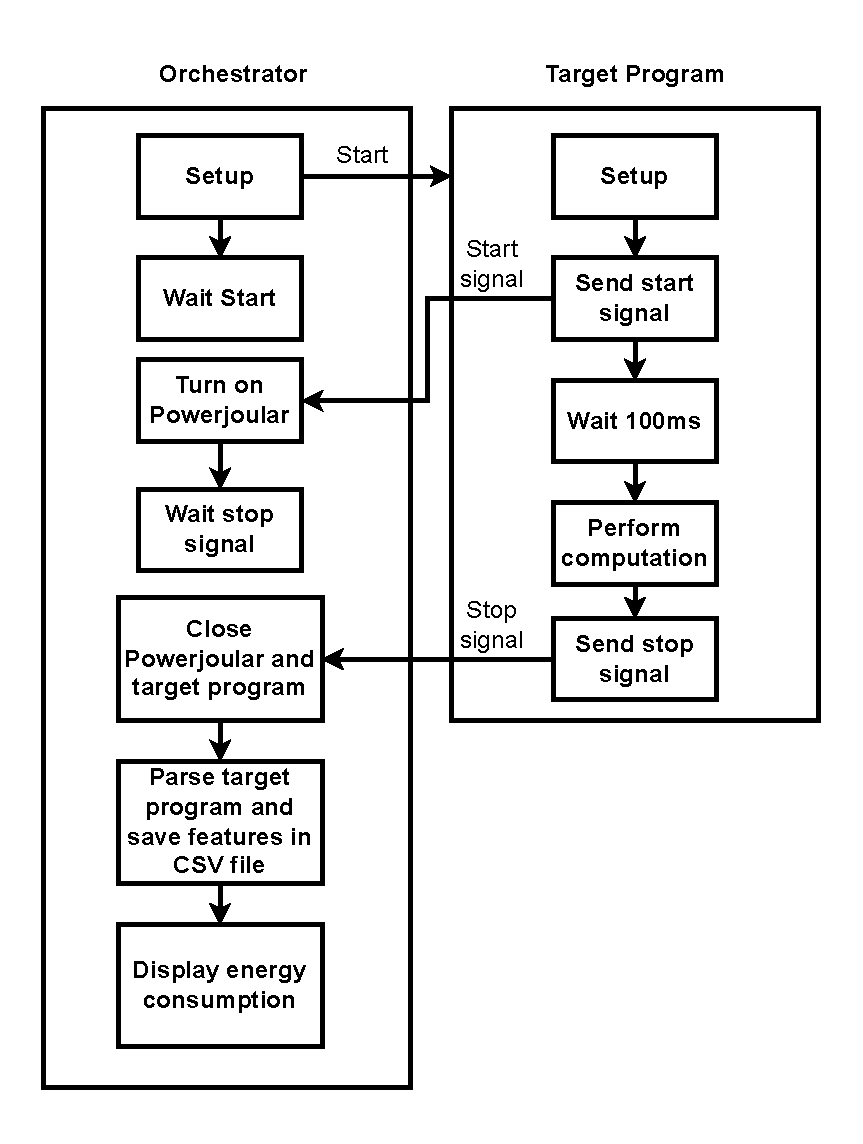
\includegraphics[width = 0.4 \textwidth]{figures/orchestrators_process.pdf}
  \caption{Orchestrator Workflow}
  \label{fig:orchestrators_process}
\end{figure}

The same workflow will be repeated across multiple machines to gather data from as many locations as possible. This approach ensures that the model developed in the next step will generate accurate outputs applicable to a wide range of machines and scenarios.

\subsection{Step 2: Energy Inference Function} \label{sec:work_step2_energy_inference_function}

\begin{figure}%[h]
  \centering
  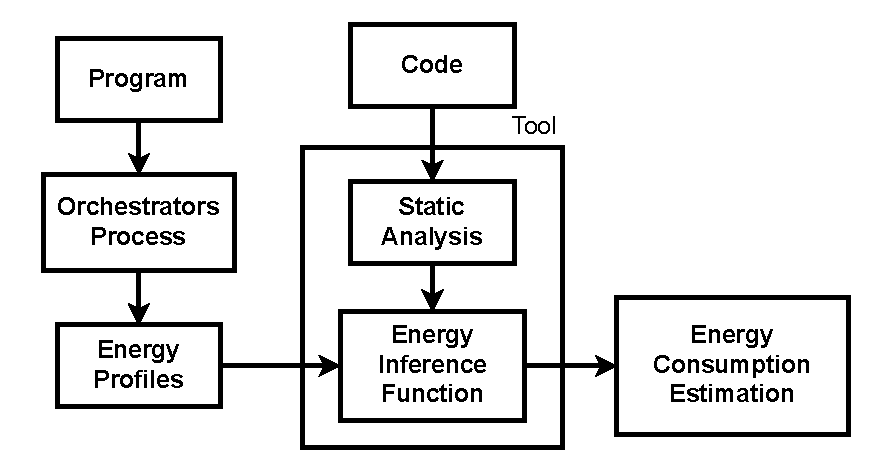
\includegraphics[width = 0.4 \textwidth]{figures/energy_inf_fun.pdf}
  \caption{Energy Inference Function}
  \label{fig:energy_inference_function}
\end{figure}

The inference function will receive as input the energy profiles obtained previously and the code that the developer wants to analyze. On receiving the code, static analyzes will be used in order to inspect the code using a Java parser (Spoon), which will provide the AST. Later this AST will be used to feed a machine learning model with the return types of the function, parameters used, loops and so on, alongside with the energy profiles. After that the model will output the estimated energy values to be displayed to the developer.
As explained in \ref{sec:background_machine_learning}, there are several ways of implementing an ML model. In this particular case, supervised ML is the best approach as it allows to train the model on previously collected energy profiles that contain the code and the energy consumed for that code. With these in mind, it is possible to test different algorithms, like the ones described in \ref{sec:background_machine_learning}, to achieve the best estimation possible.


The model will be trained using a variety of energy profiles and code inputs from different devices to achieve the most accurate energy estimates possible. This approach will improve its accuracy across devices with different hardware and software configurations.
The estimation will be the total energy used by the program, the total energy used for each function and the snippets of the function that spend the most energy.
The Figure \ref{fig:energy_inference_function} helps to visualize the function.

\subsection{Step 3: Implementation and testing} \label{sec:work_step3_implementation_and_testing}

Once the main components of the tool are built, they need to be assembled into the extension. When using it, the developers should be able to see the total energy estimate of their code in the IDE, and it should also show the estimates for each function and its most energy consuming lines.
The estimate alone may be enough to understand if the code is high or low in energy consumption, for example, if the developer has two implementations of the same function and they both give different values, it may be easy to understand which one consumes the most. However, this may not always be the case, so the tool will also provide some information to help the developer know how good or bad the energy efficiency of the code is.

Another important step is to test and ensure that the tool performs as expected on most machines, delivers the most accurate estimations possible, and undergoes a final comparison with other tools to evaluate its effectiveness.

\section{Preliminary Results} \label{sec:preliminaryresults}

In the start of the project, some tools were tested in order to see how to get the energy profiles for later use. The tools tested were PowerJoular, Powertop, Perf and JoularJx.

Perf is a Linux tool primarily designed for analyzing application performance characteristics rather than precise energy measurement. While it can provide some energy-related metrics, its measurements tend to be imprecise. In this context, Perf was used mainly to get a rough idea of energy consumption and to serve as an alternative when more accurate tools were unavailable.

Powertop was also tested, but it could only perform energy measurements on laptops, as it relies on battery drain data to calculate energy consumption. Since this approach doesn't align with our specific requirements, we considered Powertop as a last-resort option.

JoularJx is an energy measurement tool capable of measuring the consumption of Java programs and its methods. However, it is not as precise as other tools as it requires to measure the entire start of the JVM and whole functions instead of small code blocks.

As described in the \ref{sec:background_energy}, PowerJoular is the best option. As a command line program it can be easily adapted to measure any program or code snippet in most languages. So it was combined with the framework experiment-runner, that facilitates the process.

Initially, JoularJx and the experiment-runner using PowerJoular were used to explore their capabilities and familiarize with the tools. A sample Fibonacci program written in Java and C was used as a test case. However, the energy measurements provided by the two tools differed, and the experiment runner occasionally encountered errors. Later, it was determined that these problems were due to incorrect use of the framework. However, it was still decided the best approach was to make a new orchestrator similar to the Experiment-Runner, but simpler and specifically focused on measuring process energy consumption using PowerJoular. A Java-based orchestrator was initially developed because the Fibonacci implementation was also in Java. However, when tested, the energy measurement results differed significantly from those of the experiment runner, even though the main difference was the programming language (Java vs. Python).

To further analyze these inconsistencies, another orchestrator was developed in Python. This allowed for a closer examination of the differences in energy measurements and a deeper understanding of the behavior of the tools.

Using the process explained on \ref{sec:work} it was noticeable that the Java orchestrator was getting significantly more energy consumption than the Python one, which is not very logical, since they both target the same program. So, to try and check which one was having problems, two more orchestrators were implemented, one in C and another in bash.

After running the tests again it was possible to see that the Python orchestrator was getting values way more different from the other three orchestrators as show in Figure \ref{fig:4_orchs_comparison}.
The figure contains 100 runs of the Fibonacci recursive program written in Java and order by the less energy to the highest energy. And it shows the energy reads for the four different orchestrators used. The labels contain the average energy values and its standard deviation.

Further analysis of the orchestrators revealed a notable difference in behavior. When the Python orchestrator was running, both the parent and child processes consumed CPU resources. In contrast, the other orchestrators (Java, C, and Bash) showed CPU usage only in the child process. This disparity may explain why PowerJoular reported lower energy consumption for the Python orchestrator. Since the CPU load was shared between the parent and child processes, PowerJoular, which measures energy only for the child process (the target Fibonacci program), captured less total energy usage.
Since the experiment runner included an example demonstrating how to use the framework with PowerJoular, the authors were made aware of this potential conflict when launching PowerJoular from Python.

\begin{figure}%[h]
  \centering
  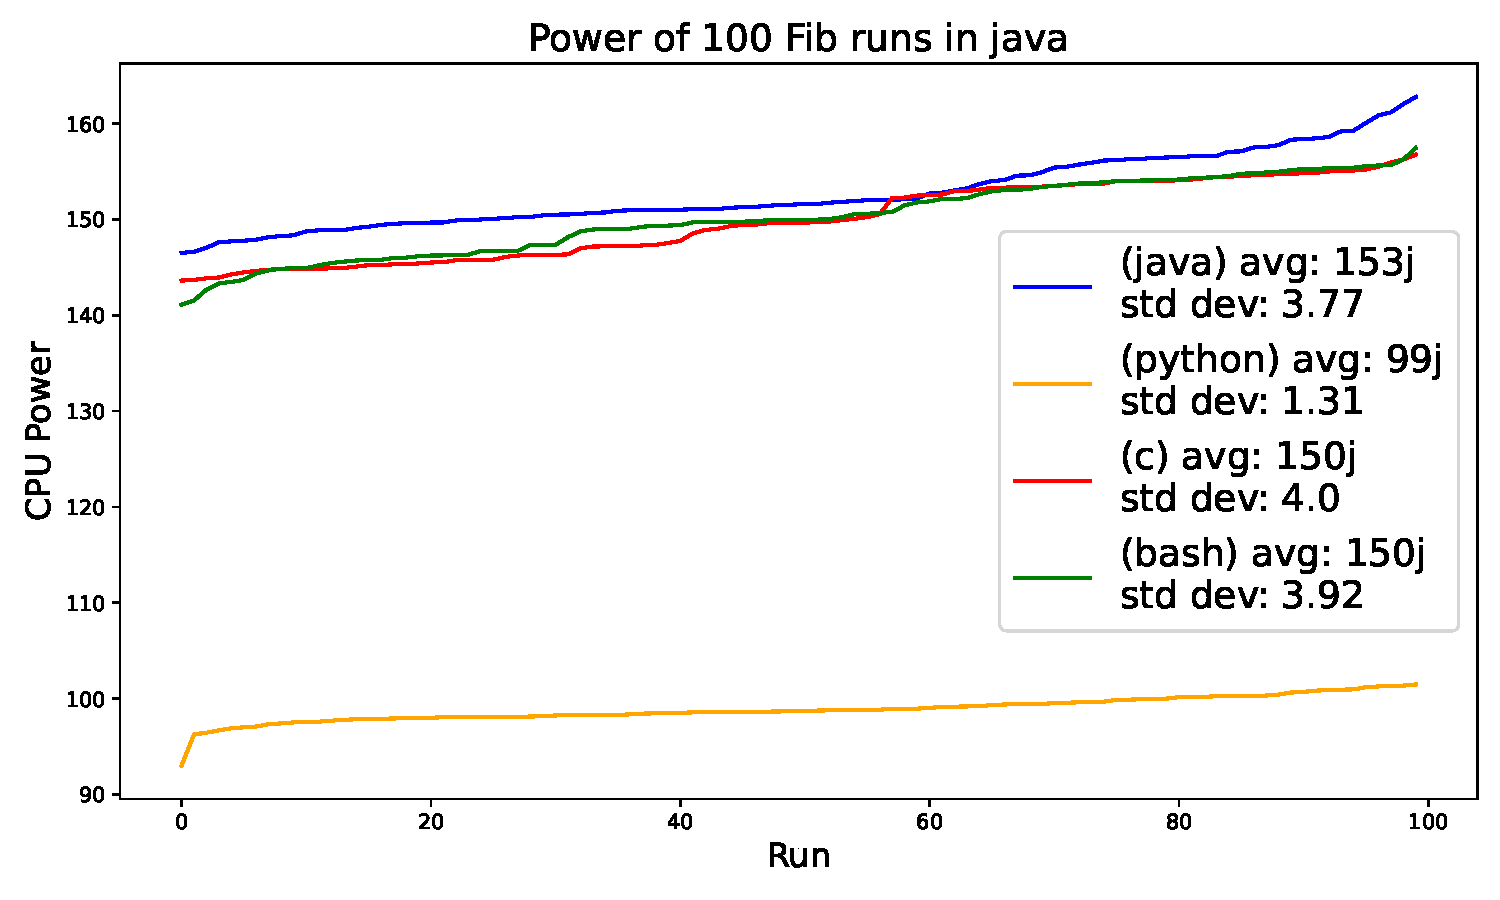
\includegraphics[width = 0.5 \textwidth]{figures/4_orchestrators_comparison.pdf}
  \caption{orchestrators comparison}
  \label{fig:4_orchs_comparison}
\end{figure}

\section{Forthcoming Work and Conclusions} \label{sec:forthcoming_work_and_conclusions}

This section explains what work will be continued to do in the thesis and present a brief conclusion on what as been done.

\subsection{Forthcoming Work}

Building on the progress made so far, additional energy profiles must be created to develop a robust energy inference function. This task involves collecting profiles from different machines and gathering enough data to effectively train the machine learning model. The static analysis tool will be implemented and used to provide important code, specifically, certain features that will feed into the model.

After that the efforts will be on developing the actual energy inference function. This task is expected to be the most time-consuming, as it is crucial to the tool functioning. It is most likely that this task overlaps the energy profiling task as more profiles might need to be collected. The task will start by implementing the ML algorithms described in \ref{sec:background_machine_learning}, test their accuracy and improving it by tuning the energy profiles for many possible cases.

When the function is completed, it will be tested against other tools to ensure its quality. The extension will then be built and tested in IDEs.
While developing the function and the extension, the writing of the thesis will also be done in parallel documenting every information.

\begin{figure*}%[h]
  \centering
  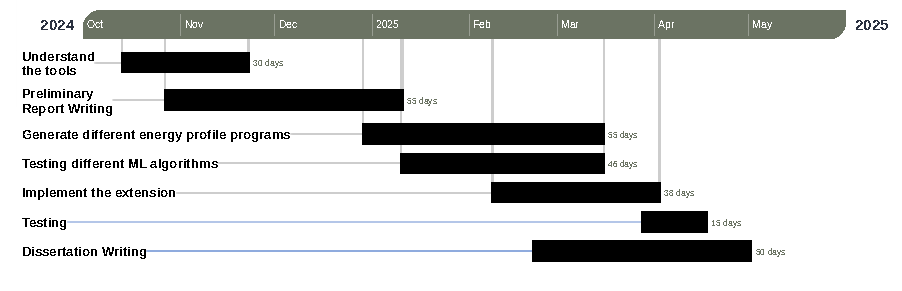
\includegraphics[width = 1 \textwidth]{figures/gantt_diagram.pdf}
  \caption{Work Plan}
  \label{fig:gantt_diagram}
\end{figure*}


The work plan is illustrated more clearly in Figure \ref{fig:gantt_diagram}, which provides a visual representation of the described tasks. While the dates shown in the figure may not precisely align with the actual timeline, the sequence of tasks remains accurate.

\subsection{Conclusion}

The techniques and tools in past and recent research have been studied, and this work improves on those different research and tools, by providing an easy-to-use tool that is also easy accessible and provides energy estimations.
For now, the tool to perform the energy profiling as been selected, (PowerJoular) and a process to create the profiles has been made. This process, as explained in section \ref{sec:work_step1_energy_profiling}, allows targeting specific parts of programs, or the entire program, measure the energy consumption and extract important features. The selection of the tools had some setbacks. When testing PowerJoular it was noticed that it didn't work correctly when using python as an orchestrator, obtaining different measurements than the other orchestrators, (Java, C, Bash), as explained in section \ref{sec:preliminaryresults}. Other than that, the tool worked fine, and it's capable of completing its task of energy profiling. The next step is to start the development of the energy inference function, by collecting the required data. When completed, it is expected that the tool can raise energy awareness among developers, and help facilitate the process of making energy efficient code.


%It should include subsections that describe the work to be carried out during the rest of the year, and what its objectives are.
%
%It should also include planning until the end of the work, in chronological order.
%
%Include a final concluding subsection (may be a separate section) with a summary of contributions already made, a preliminary self-assessment of the work done so far, and difficulties encountered.


%%%%%%%%%%%%%%%%%%%%%%%%%%%%%%%%%%%%%%%%%%%%%%%%%%%%%%%%%%%%%%%%%%%%%%
%% The next two lines define the bibliography style to be used, and
%% the bibliography file.
\bibliographystyle{unsrt}
\bibliography{ref}
\end{document}
